%\documentclass{article}
\documentclass[border=5pt]{standalone}
\usepackage{my_packages}
\usepackage{tikz}
\usetikzlibrary{3d}

\tikzset{help lines/.style={very thin,color=gray!50}} % modify the help lines style

 \makeatletter
 \tikzoption{canvas is xy plane at z}[]{%
   \def\tikz@plane@origin{\pgfpointxyz{0}{0}{#1}}%
   \def\tikz@plane@x{\pgfpointxyz{1}{0}{#1}}%
   \def\tikz@plane@y{\pgfpointxyz{0}{1}{#1}}%
   \tikz@canvas@is@plane
 }
 \makeatother  

  
\begin{document}

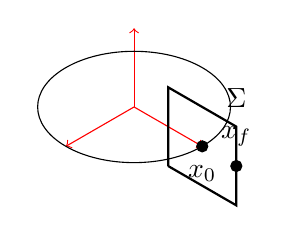
\begin{tikzpicture}[x={(-0.866cm,-0.5cm)}, y={(0.866cm,-0.5cm)}, z={(0cm,1cm)}, scale=1]
	% draw 3d axis

	\draw[->,red] (0,0,0) --  (1,0,0);
  	\draw[->,red] (0,0,0) --  (0,1,0);    
  	\draw[->,red] (0,0,0) --  (0,0,1);

    % draw circle in xy plane z=1.5
    \begin{scope}[canvas is xy plane at z=0]
        \node[label=below:\(\vecbf{x}_{0}\)] (x0) at (0,1) {\pgfuseplotmark{*}};
        \node[label=above:\(\vecbf{x}_{f}\)] (x0) at (0,1.5) {\pgfuseplotmark{*}};
        \node[] (xm) at (0,-1) {};
        \draw [black] (0,0) circle (1);
    \end{scope}

  	% draw yz plane Poincare section
  	\begin{scope}[canvas is yz plane at x=0]
  		\node[label=above:\(\Sigma\)] (upper_right) at (1.5,0.5) {};
        \node[] (upper_left) at (0.5,0.5) {};
        \node[] (lower_left) at (0.5,-0.5) {};
        \node[] (lower_right) at (1.5,-0.5) {};

      	\draw[black, thick] (lower_left.center) -- (lower_right.center)--(upper_right.center) --(upper_left.center)-- (lower_left.center);
  	\end{scope}  

\end{tikzpicture}


\end{document}